\section{Experimental details on the Waterbirds dataset}
\label{sec:waterbirds}
In this section, we discuss the experimental details and construction of the Waterbirds dataset in more detail. We also provide ablation studies of attack parameters such as the size of the motion blur kernel, plots of the robust error decomposition with increasing $\numsamp$, and some experiments using early stopping.

\paragraph{The waterbirds dataset}

To build the Waterbirds dataset, we use the CUB-200 dataset \cite{Welinder10}, which contains images and labels of $200$ bird species, and $4$ background classes (forest, jungle/bamboo, water ocean, water lake natural) of the Places dataset \cite{zhou17}.The aim is to recognize whether or not the bird, in a given image, is a waterbird (e.g. an albatros) or a landbird (e.g. a woodpecker). To create the dataset, we randomly sample equally many water- as landbirds from the CUB-200 dataset. Thereafter, we sample for each bird image a random background image. Then, we use the segmentation provided in the CUB-200 dataset to segment the birds from their original images and paste them onto the randomly sampled backgrounds. The resulting images have a size of $256 \times 256$. Moreover, we also resize the segmentations such that we have the correct segmentation profiles of the birds in the new dataset as well. For the concrete implementation, we use the code provided by \cite{Sagawa20}.

\paragraph{Experimetal training details}
Following the example of \cite{Sagawa20}, we use a ResNet50 pretrained on the ImageNet dataset for all experiments, a weight-decay of $10^{-4}$, and train for $300$ epochs using the Adam optimizer. Extensive fine-tuning of the learning rate resulted in an optimal learning rate of $0.006$ for all experiments in the low sample size regime. Adversarial training is implemented as suggested in \cite{madry18}: at each iteration we find the worst case perturbation with an exact or approximate method. In all our experiments, the resulting classifier interpolates the training set. We plot the mean over all runs and the standard deviation of the mean. 

\paragraph{Specifics to the motion blur attack}
Fast moving objects or animals are hard to photograph due to motion blur. Hence, when trying to classify or detect moving objects from images, it is imperative that the classifier is robust against reasonable levels of motion blur. We implement the attack as follows. First, we segment the bird from the original image, then use a blur filter and lastly, we paste the blurred bird back onto the background. We are able to apply more severe blur, by enlarging the kernel of the filter. See Figure \ref{fig:motion_blur_panel} for an ablation study of the kernel size. 

The motion blur filter is implemented as follows. We use a kernel of size $\motionblurkernel \times \motionblurkernel$ and build the filter as follows: we fill the row $(\motionblurkernel-1)/2$ of the kernel with the value $1/\motionblurkernel$. Thereafter, we use the 2D convolution implementation of OpenCV (filter2D) \cite{opencv_library} to convolute the kernel with the image. Note that applying a rotation before the convolution to the kernel, changes the direction of the resulting motion blur. Lastly, we find the most detrimental level of motion blur using a list-search over all levels up to $\motionblurkernel_{max}$. 


\begin{figure*}[!t]
\centering
\begin{subfigure}[b]{0.19\textwidth}
  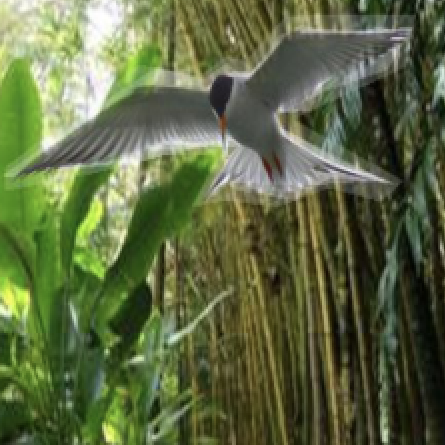
\includegraphics[width=0.99\linewidth]{plotsAistats/waterbird_original_example.png}
  \caption{Original}
  \label{fig:motion_blur_or}
\end{subfigure}
\begin{subfigure}[b]{0.19\textwidth}
  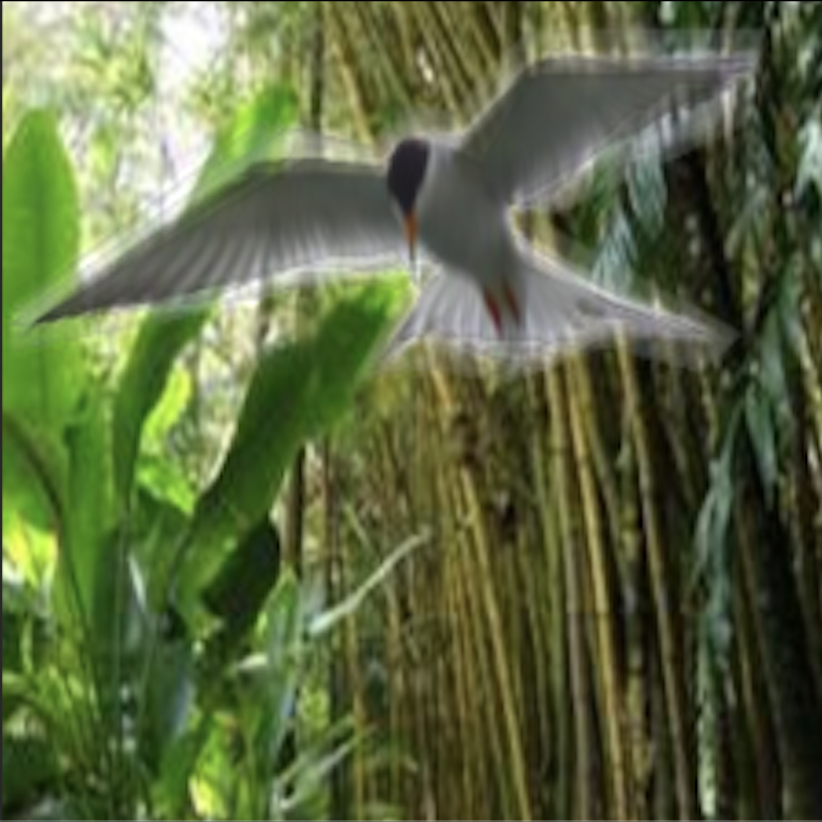
\includegraphics[width=0.99\linewidth]{plotsAistats/motion_blur_5.png}
  \caption{$\motionblurkernel = 5$}
  \label{fig:motion_blur_5}
\end{subfigure}
\begin{subfigure}[b]{0.19\textwidth}
  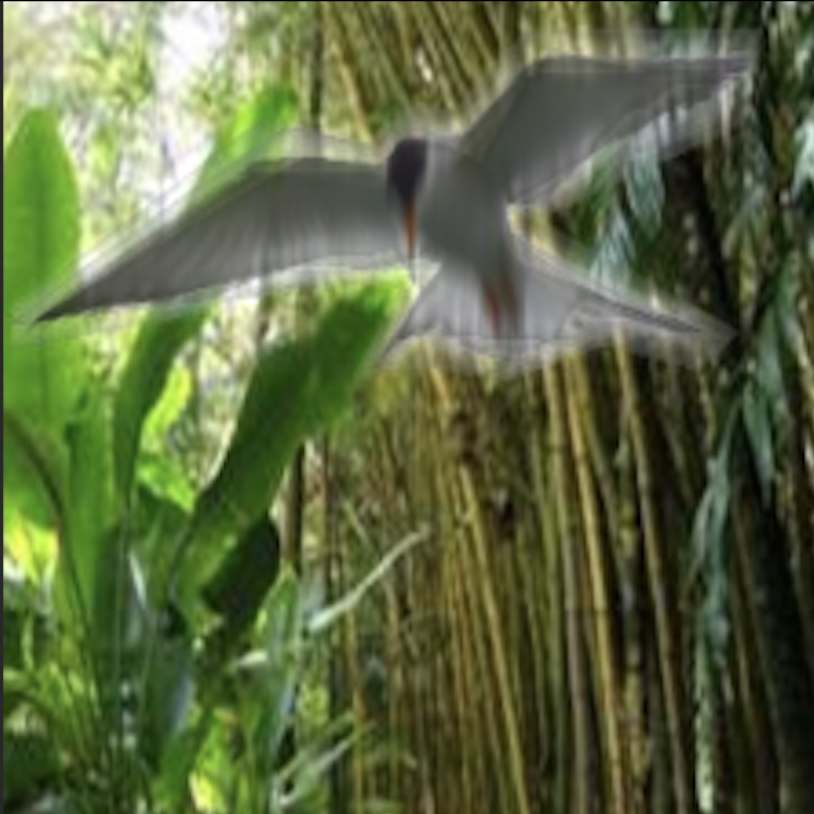
\includegraphics[width=0.99\linewidth]{plotsAistats/motion_blur_10.png}
  \caption{$\motionblurkernel = 10$}
  \label{fig:motion_blur_10}
\end{subfigure}
\begin{subfigure}[b]{0.19\textwidth}
  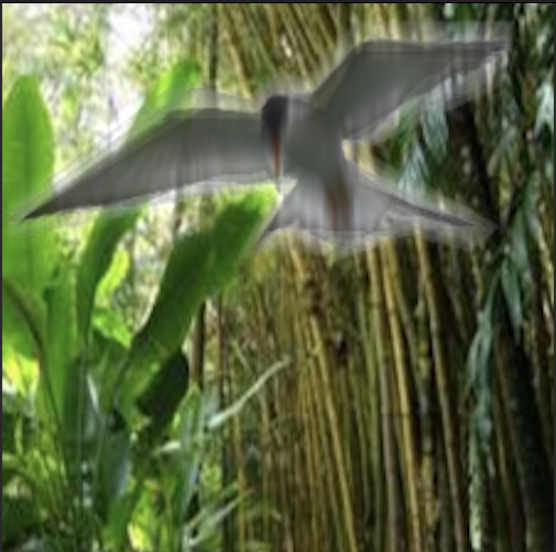
\includegraphics[width=0.99\linewidth]{plotsAistats/motion_blur_15.png}
  \caption{$\motionblurkernel = 15$}
  \label{fig:motion_blur_15}
\end{subfigure}
\begin{subfigure}[b]{0.19\textwidth}
  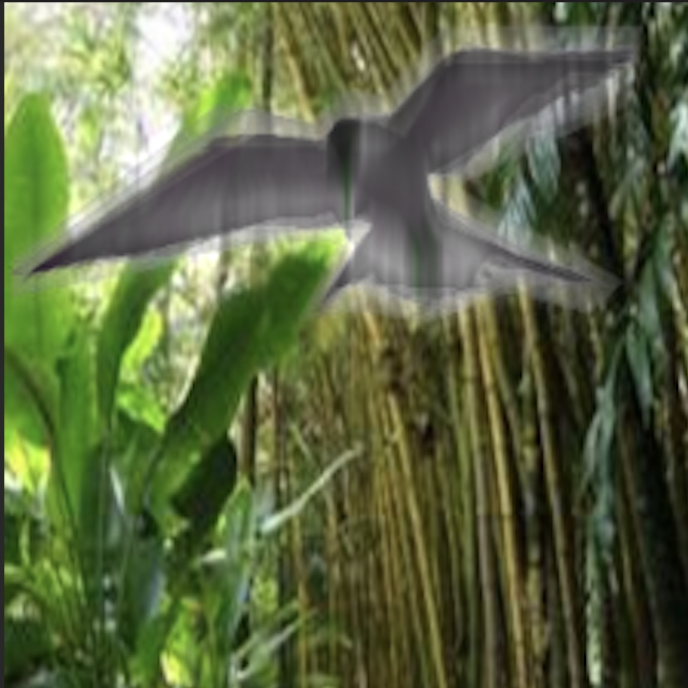
\includegraphics[width=0.99\linewidth]{plotsAistats/motion_blur_20.png}
  \caption{$\motionblurkernel = 20$}
  \label{fig:motion_blur_20}
\end{subfigure}
\caption{We perform an ablation study of the motion blur kernel size, which corresponds to the severity level of the blur. We see that for increasing $\motionblurkernel$, the severity of the motion blur increases. In particular, note that for $\motionblurkernel = 15$ and even $\motionblurkernel = 20$, the bird remains recognizable: we do not semantically change the class, i.e. the perturbations are consistent.}
\label{fig:motion_blur_panel}
\end{figure*}

\begin{figure*}[!b]
\centering
\begin{subfigure}[b]{0.136\textwidth}
  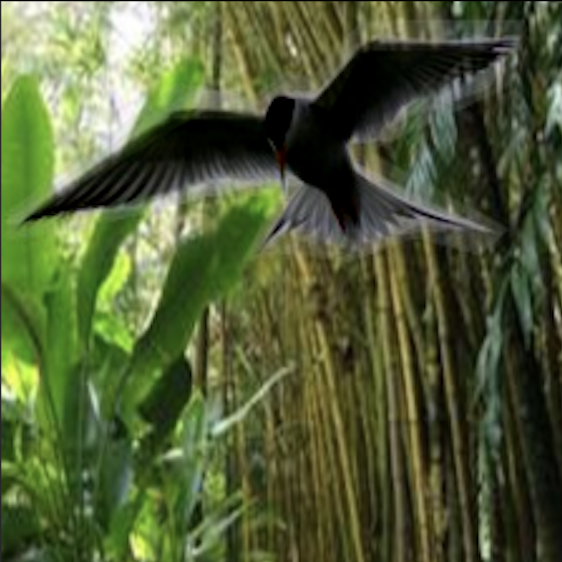
\includegraphics[width=0.99\linewidth]{plotsAistats/bird_light_03_dark.png}
  \caption{$\epsilon = -0.3$}
  \label{fig:dark_03}
\end{subfigure}
\begin{subfigure}[b]{0.136\textwidth}
  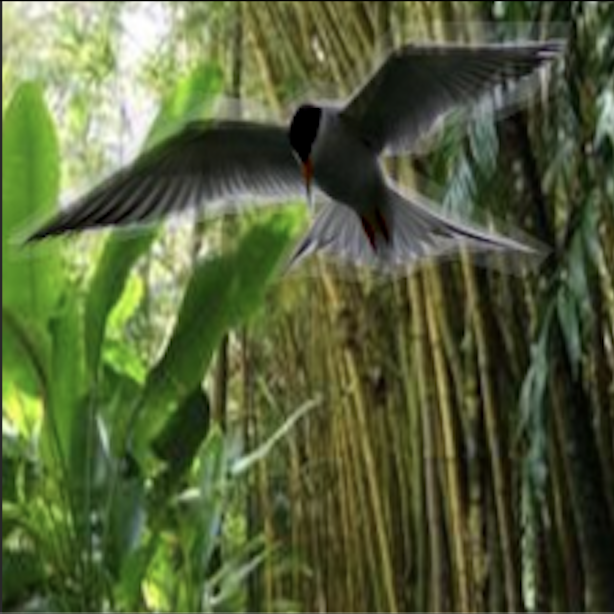
\includegraphics[width=0.99\linewidth]{plotsAistats/bird_light_02_dark.png}
  \caption{$\epsilon = -0.2$}
  \label{fig:dark_02}
\end{subfigure}
\begin{subfigure}[b]{0.136\textwidth}
  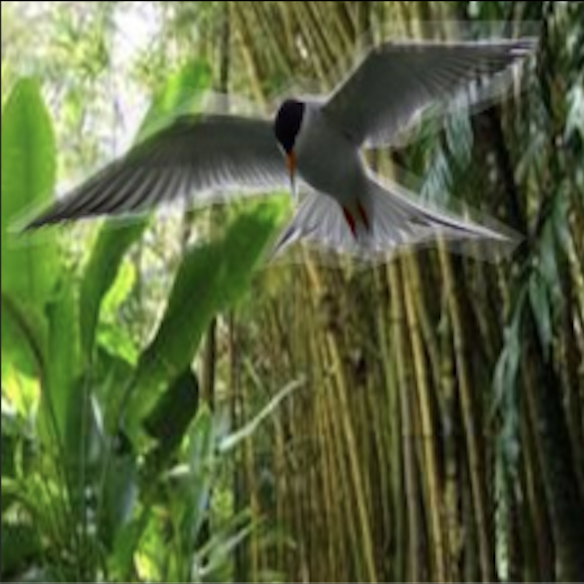
\includegraphics[width=0.99\linewidth]{plotsAistats/bird_light_01_dark.png}
  \caption{$\epsilon = -0.1$}
  \label{fig:dark_01}
\end{subfigure}
\begin{subfigure}[b]{0.136\textwidth}
  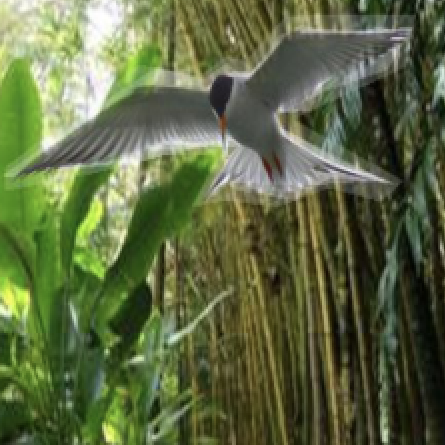
\includegraphics[width=0.99\linewidth]{plotsAistats/waterbird_original_example.png}
  \caption{Original}
  \label{fig:light_or}
\end{subfigure}
\begin{subfigure}[b]{0.136\textwidth}
  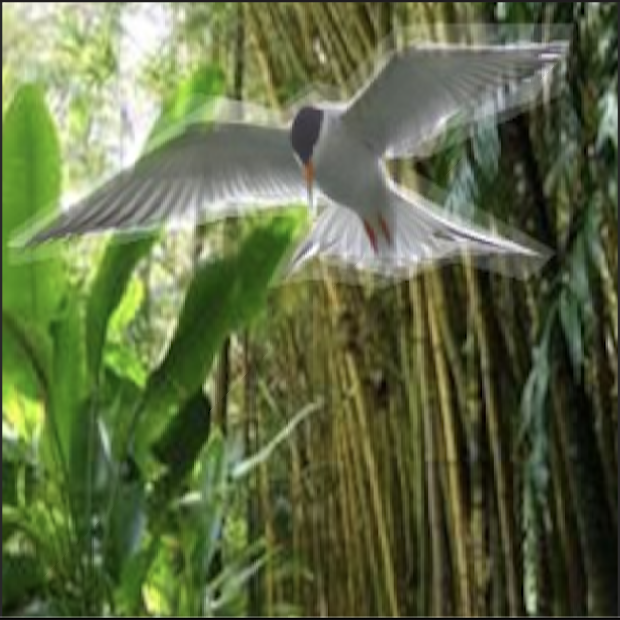
\includegraphics[width=0.99\linewidth]{plotsAistats/bird_light_01_light.png}
  \caption{$\epsilon = 0.1$}
  \label{fig:light_01}
 \end{subfigure}
\begin{subfigure}[b]{0.136\textwidth}
  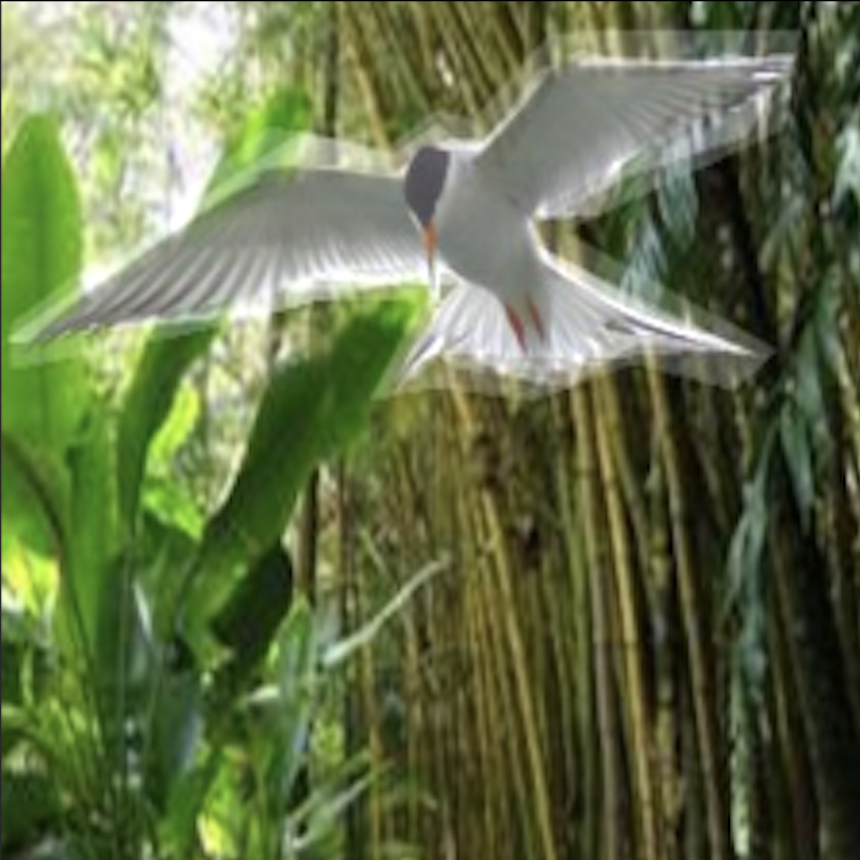
\includegraphics[width=0.99\linewidth]{plotsAistats/bird_light_02_light.png}
  \caption{$\epsilon = 0.2$}
  \label{fig:light_02}
\end{subfigure}
\begin{subfigure}[b]{0.136\textwidth}
  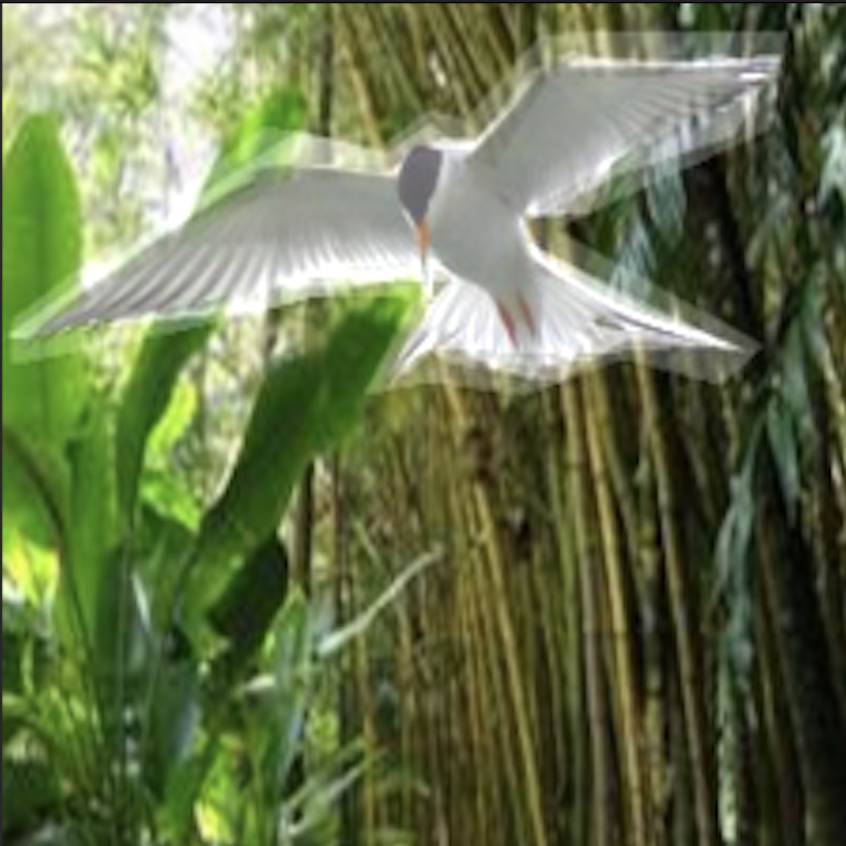
\includegraphics[width=0.99\linewidth]{plotsAistats/bird_light_03_light.png}
  \caption{$\epsilon = 0.3$}
  \label{fig:light_03}
\end{subfigure}
\caption{We perform an ablation study of the different lighting changes of the adversarial illumination attack. Even though the \nameofattack attacks the signal component in the image, the bird remains recognizable in all cases.}
\label{fig:light_panel}
\end{figure*}

\paragraph{Specifics to the adversarial illumination attack} 
An adversary can hide objects using poor lightning conditions, which can for example arise from shadows or bright spots. To model poor lighting conditions on the object only (or targeted to the object), we use the adversarial illumination attack. 
The attack is constructed as follows: First, we segment the bird from their background. Then we apply an additive constant $\epsilon$ to the bird, where the absolute size of the constant satisfies $|\epsilon| < \epstest = 0.3$. Thereafter, we clip the values of the bird images to $[0, 1]$, and lastly, we paste the bird back onto the background. See Figure \ref{fig:light_panel} for an ablation of the parameter $\epsilon$ of the attack. It is non-trivial how to (approximately) find the worst perturbation. We find an approximate solution by searching over all perturbations with increments of size $\epstest/K_{\text{max}}$. Denote by \segmentation, the segmentation profile of the image $x$. We consider all perturbed images in the form of
\begin{equation*}
x_{pert} = (1-seg) x + seg (x + \epsilon \frac{K}{K_{\text{max}}}  1_{255 \times 255}), \Hquad K \in [-K_{max}, K_{max}].
\end{equation*} 
During training time we set $K_{max} = 16$ and therefore search over $33$ possible images. During test time we search over $65$ images ($K_{max} = 32$).

\paragraph{Early stopping} In all our experiments on the Waterbirds dataset, a parameter search lead to an optimal weight-decay and learning rate of $10^{-4}$ and $0.006$ respectively. Another common regularization technique is early stopping, where one stops training on the epoch where the classifier achieves minimal robust error on a hold-out dataset. To understand if early stopping can mitigate the effect of adversarial training aggregating robust generalization in comparison to standard training, we perform the following experiment. On the Waterbirds dataset of size $n = 20$ and considering the adversarial illumination attack, we compare standard training with early stopping and adversarial training $(\epstrain = \epstest = 0.3)$ with early stopping. Considering several independent experiments, early stopped adversarial training has an average robust error of $33.5$ a early stopped standard training $29.1$. Hence, early stopping does decrease the robust error gap, but does not close it. 

\paragraph{Error decomposition with increasing $n$}

In Figure \ref{fig:waterbirds_light_numobs}, we see that adversarial training hurts robust generalization in the small sample size regime. For completeness, we plot the robust error composition for adversarial and standard training in Figure \ref{fig:light_numsamp_decomposition}. We see that in the low sample size regime, the drop in susceptibility that adversarial training achieves in comparison to standard training, is much lower than the increase in standard error. Conversely, in the high sample regime, the drop of susceptibility from adversarial training over standard training is much bigger than the increase in standard error. 

\begin{figure*}[!t]
\centering
\begin{subfigure}[b]{0.32\textwidth}
  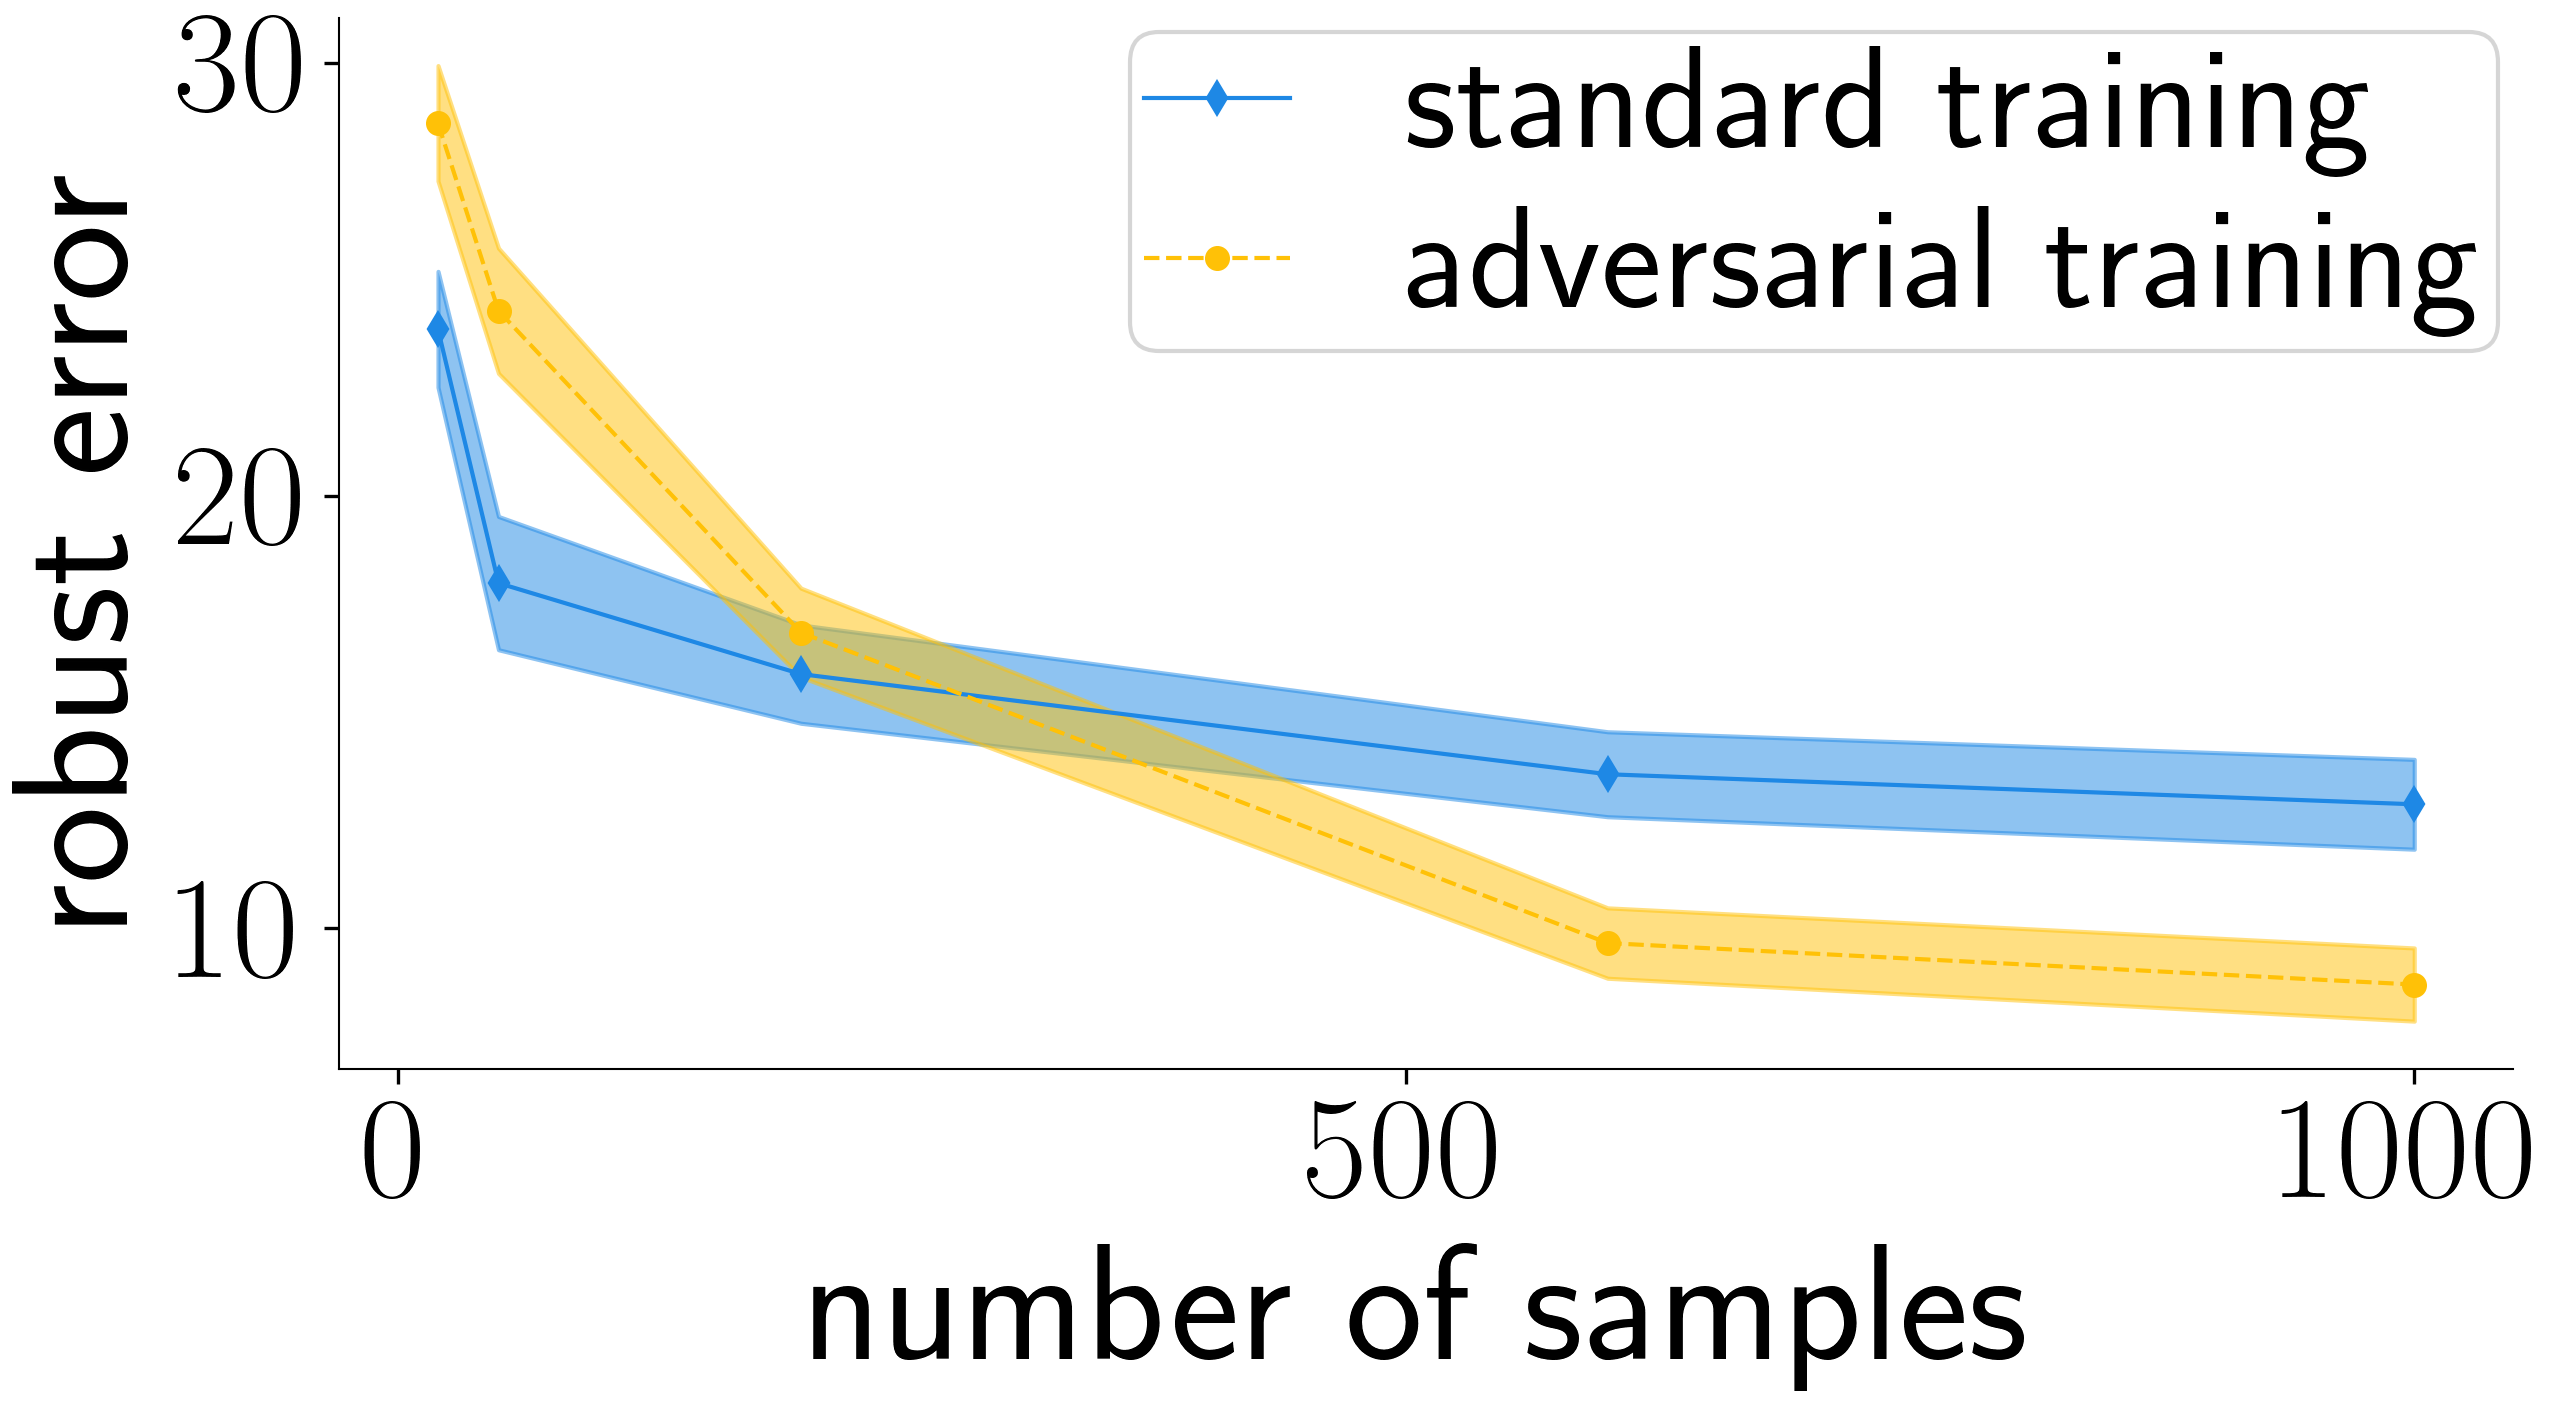
\includegraphics[width=0.99\linewidth]{plotsAistats/numsamp_waterbirds_light.png}
  \caption{Robust error}
  \label{fig:app_waterbirds_robust_error}
\end{subfigure}
\begin{subfigure}[b]{0.32\textwidth}
  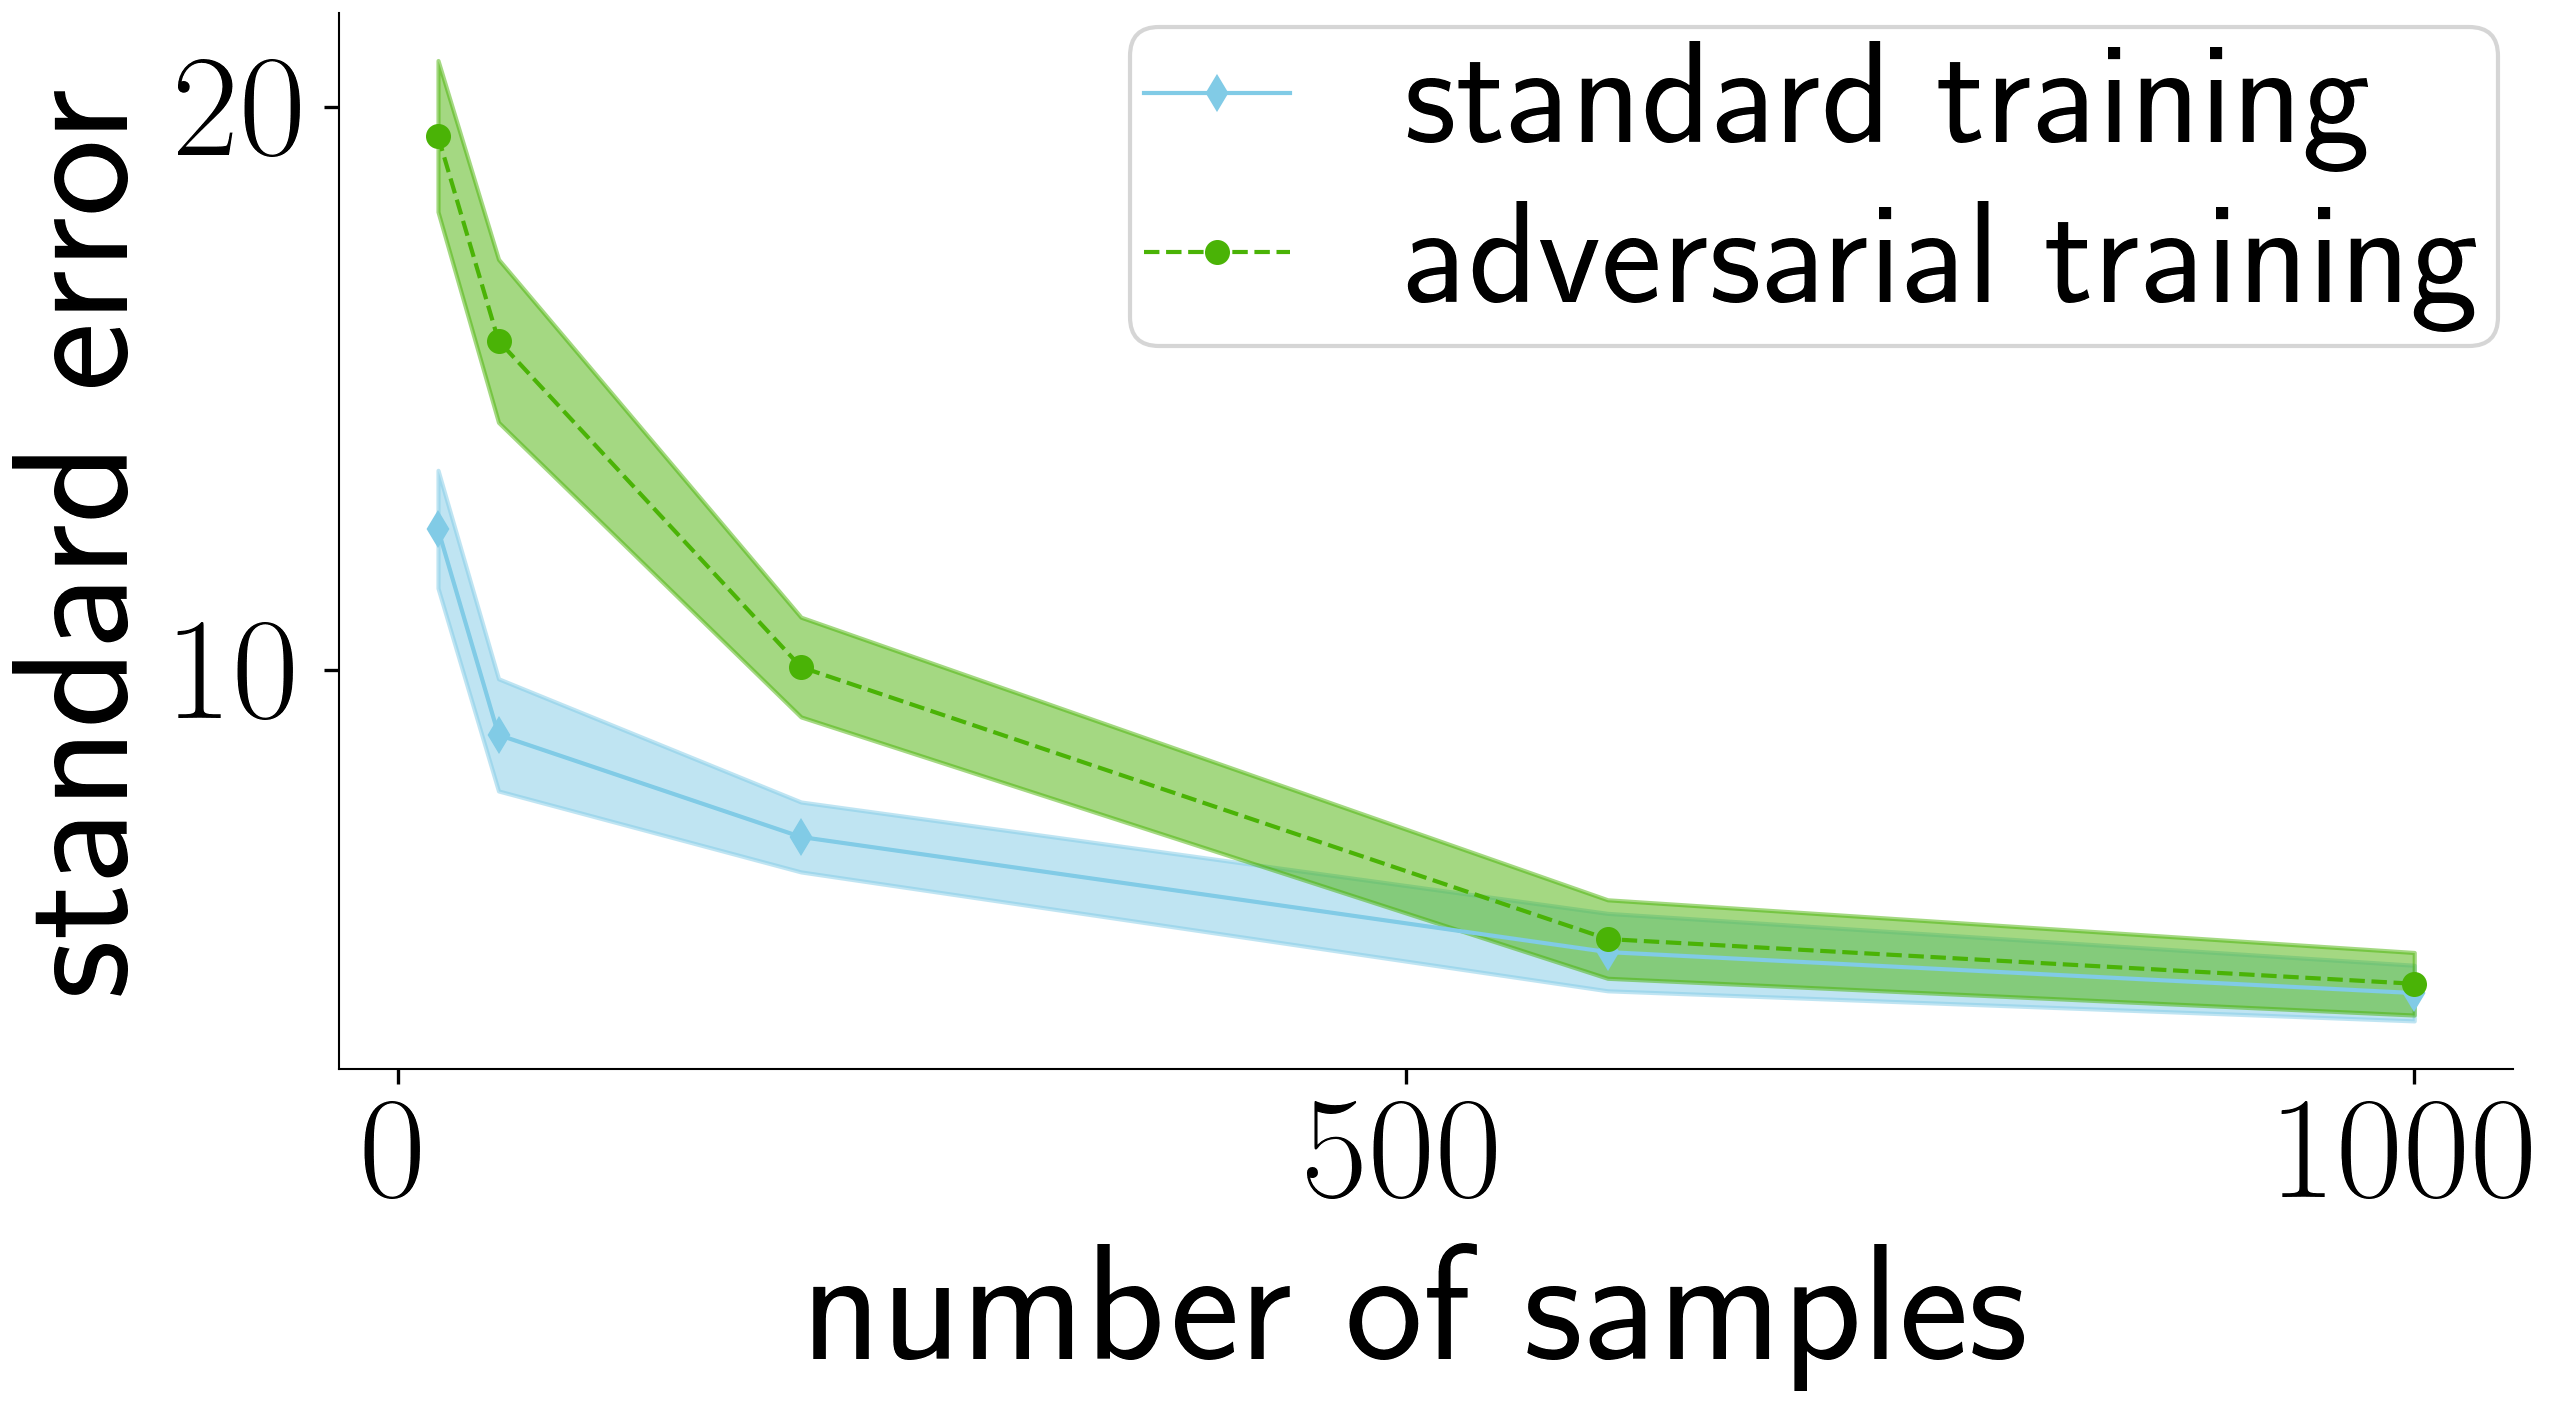
\includegraphics[width=0.99\linewidth]{plotsAistats/waterbirds_standard_numsamp.png}
  \caption{Standard error}
  \label{fig:app_waterbirds_standard_error}
\end{subfigure}
\begin{subfigure}[b]{0.32\textwidth}
  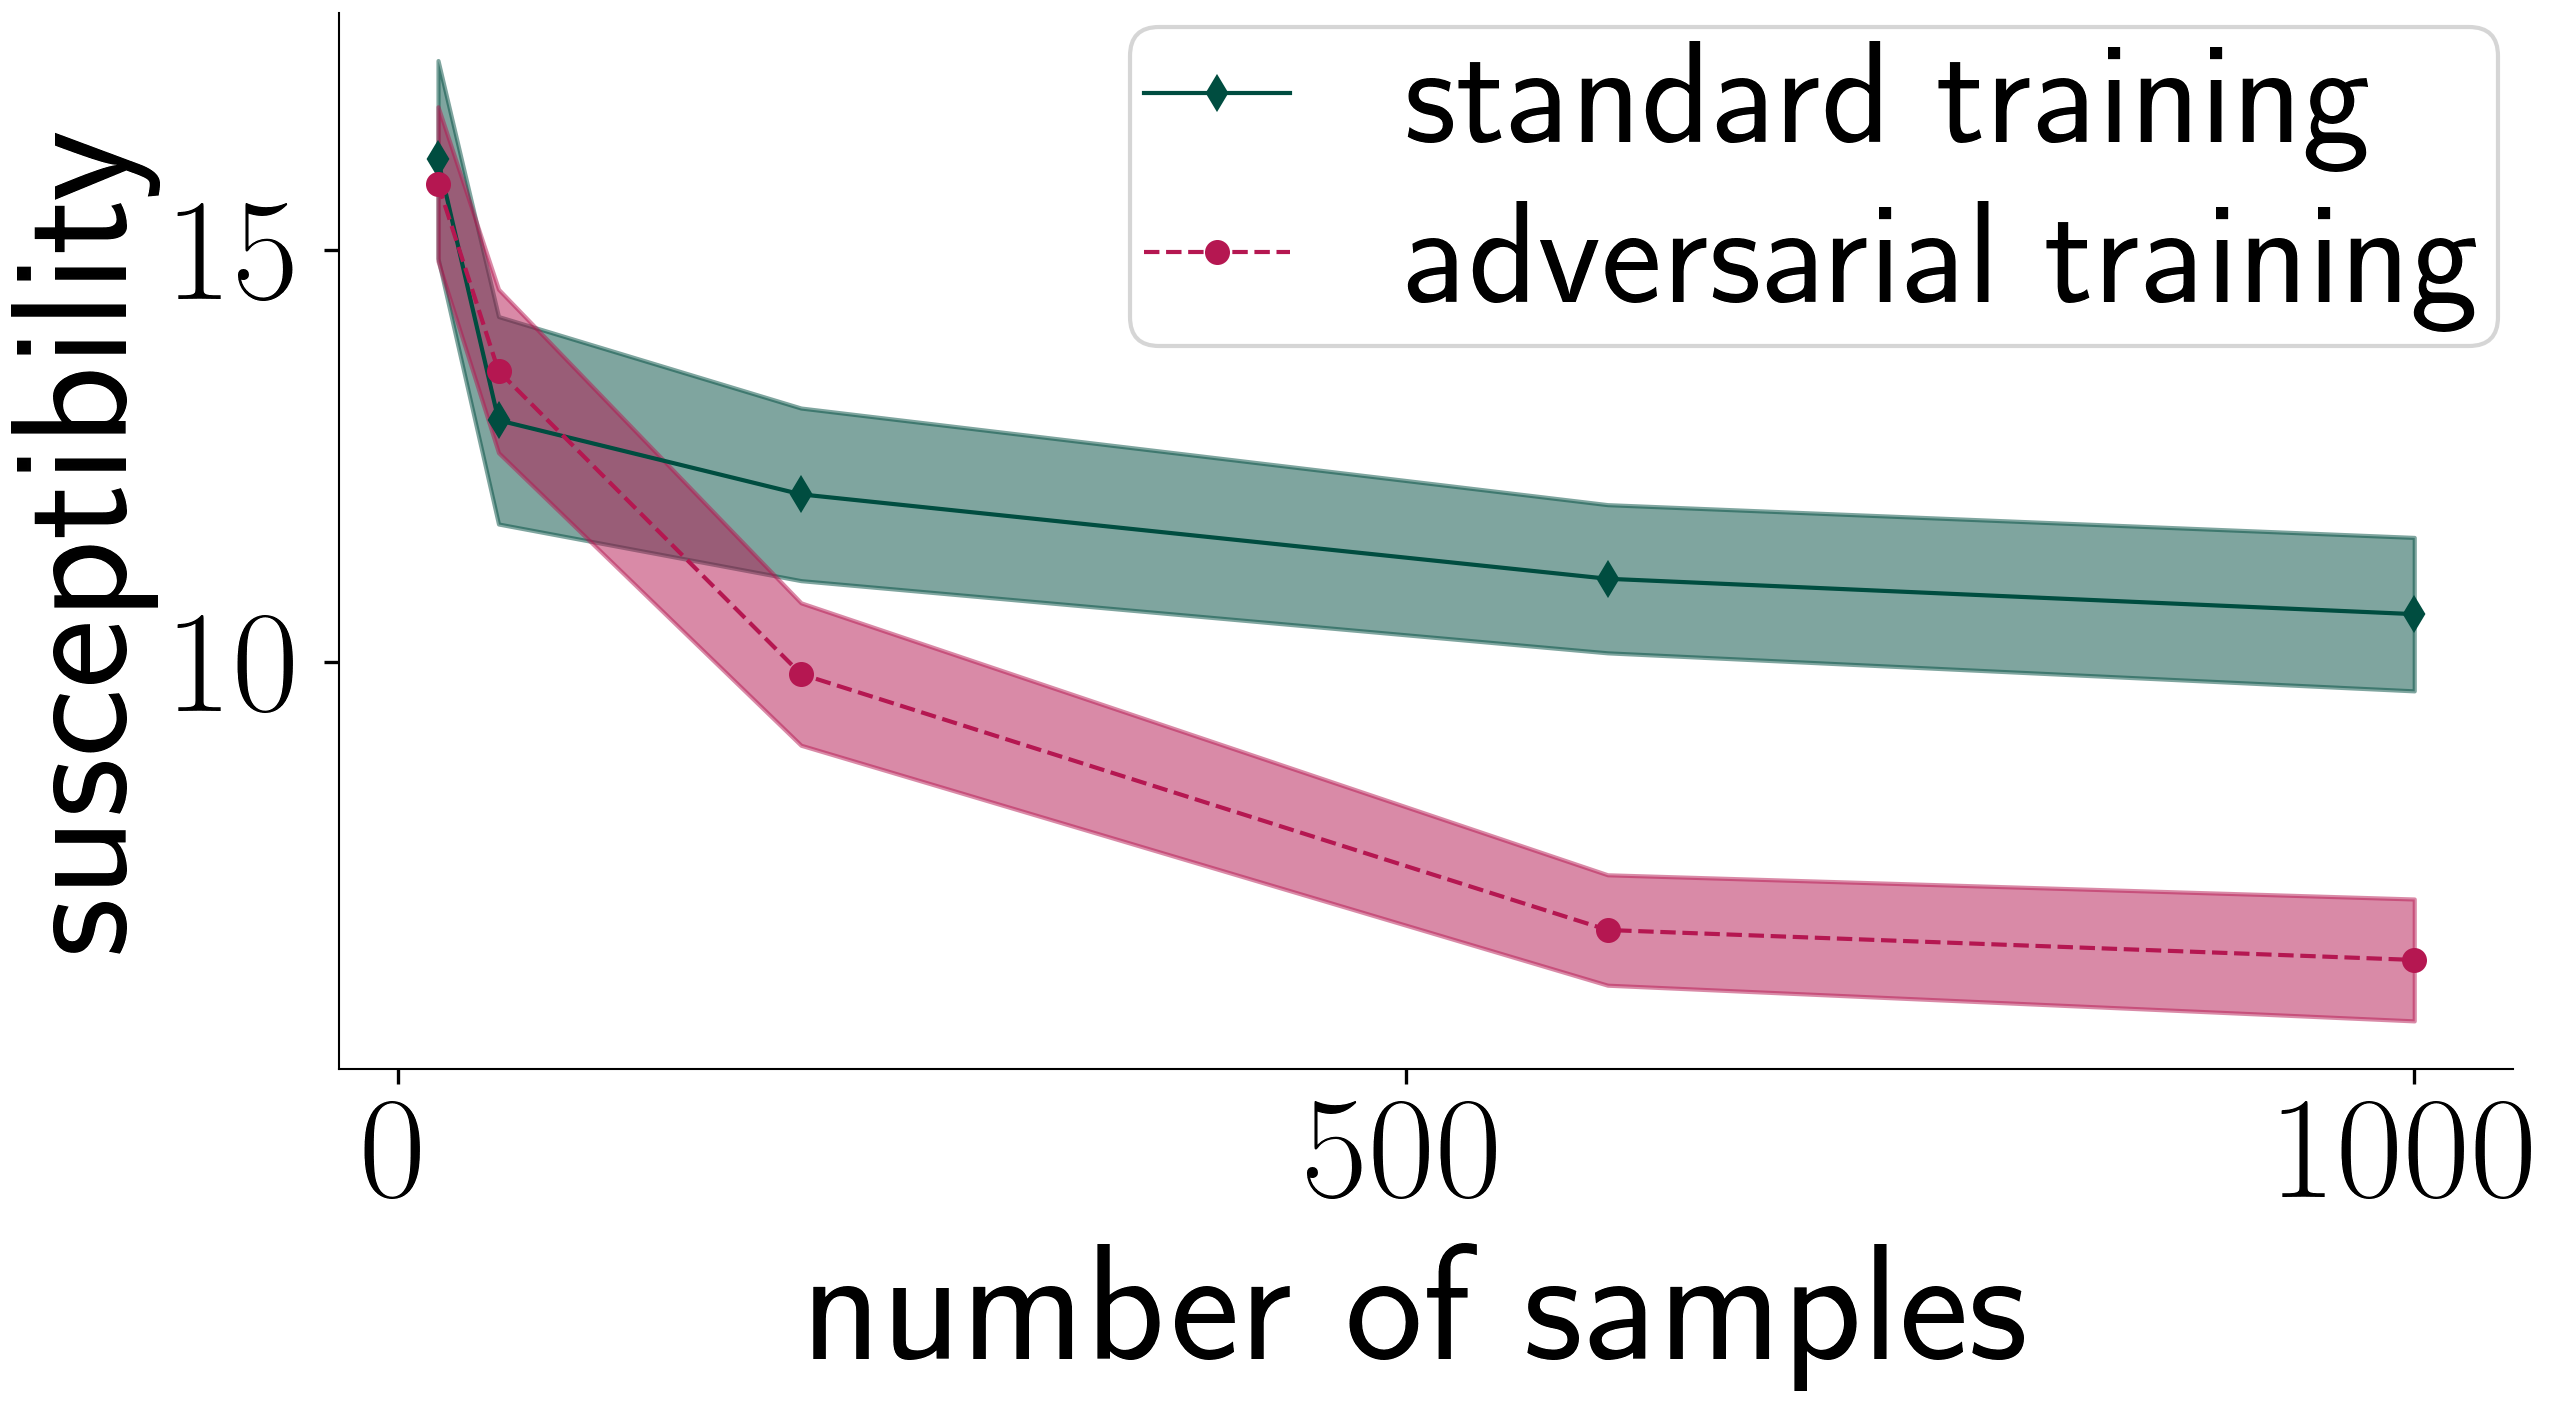
\includegraphics[width=0.99\linewidth]{plotsAistats/waterbirds_susceptibility_decomposition.png}
  \caption{Susceptibility}
  \label{fig:app_waterbirds_susceptibility}
\end{subfigure}
\caption{We plot the robust error decomposition of the experiments depicted in Figure \ref{fig:waterbirds_light_numobs}. The plots depict the mean and standard deviation of the mean over several independent experiments. We see that, in comparison to standard training, the reduction in susceptibility for adversarial training is minimal in the low sample size regime. Moreover, the increase in standard error of adversarial training is quite severe, leading to an overall increase in robust error in the low sample size regime.}
\label{fig:light_numsamp_decomposition}
\end{figure*}